\documentclass{uspBeamer}

%============================================================
%-------------------------- SETUP ---------------------------
%============================================================

\author[Silva, J. T.]{Jonathan Tobias da Silva}
\title[Detecção de intrusão em redes OPC UA utilizando ML]{Desenvolvimento de um método de detecção de intrusão em redes OPC UA baseado em técnicas de Aprendizagem de Máquinas}
\subtitle{Proposta inicial de mestrado em Engenharia Elétrica}
\institute[USP]{EESC/SEL/USP}
\date{\today}
\def \advisor{Prof. Dr. Ivan Nunes da Silva}
\def \supervisor{Prof. Dr. André Luis Dias}
\subject{USP Presentation}
\graphicspath{ {Public/Images/} }

%============================================================
%----------------------- LOCAL CONFIG -----------------------
%============================================================

\titlegraphic{
	\begin{tikzpicture}[overlay, remember picture]
		\node[right=0.9cm] at (current page.205){ % right=0.2cm - good as well
			
\includegraphics[width=60pt]{logo_eesc_horizontal-transparente.png}
		};
	\end{tikzpicture}
}
\usebackgroundtemplate{
	
\includegraphics[width=\paperwidth,height=\paperheight]{bodyEESC2.png}
}

%________________________________________________________
%--------- CRONOGRAMA ---------
\newcommand*{\thead}[1]{\multicolumn{1}{|c|}{\bfseries #1}}
\newcommand{\x}[1]{\cellcolor{mainColor1} #1}
\newcommand{\y}[1]{\cellcolor{mainColor2} #1}
%\def\arraystretch{1}
\setlength\tabcolsep{2pt}

%============================================================
%------------------------- DOCUMENT -------------------------
%============================================================

\begin{document}
	
    %________________________________________________________
	%-------------------- INIT PAGE -------------------------

    {
		\usebackgroundtemplate{
\includegraphics[width=\paperwidth,height=\paperheight]{titleEESC.png}}
		\begin{frame}[plain]
		\end{frame}
	}

	%________________________________________________________
	%-------------------- TITLE PAGE ------------------------
	
	{
		\usebackgroundtemplate{
\includegraphics[width=\paperwidth,height=\paperheight]{backgroundEESC.png}}
		\begin{frame}[plain]
			\maketitle
		\end{frame}
	}
	
	%________________________________________________________
	%------------------- TOC - PART  ------------------------

	% \part{Demonstrativa de elementos}
	\begin{frame}{Agenda}
		\tableofcontents
	\end{frame}
	
    \section{Apresentação}
    \begin{frame}{Trabalhos desenvolvidos}
        \begin{columns}
            \begin{column}{.6\textwidth}
                \begin{wideitemize}
                    \item Softwares WEB-based
                    \item Diagnóstico de falhas
                    \item \textit{Machine Learning}
                    \item Sistemas inteligentes
                    \item \textit{Cloud Computing}
                    \item Publicações
                \end{wideitemize}
            \end{column}
            \begin{column}{.4\textwidth}
                \begin{figure}
                    
\includegraphics[scale=0.6]{triplice.png}
                \end{figure}
            \end{column}
        \end{columns}
    \end{frame}

    \section{Sobre o tema}
    \begin{frame}{Motivação e Justificativa}
        \begin{columns}
            \begin{column}{.5\textwidth}
                \begin{wideitemize}
                    \uncover<1->{\item Aumento nos casos de ataques cibernéticos em CPPSs}
                    \uncover<2>{
                    \item \textit{Industrial Internet of Things}
                    \item \textit{Artificial Intelligence}
                    \item \textit{Service Orientated Architecture} (SOA)
                    \item \textit{Open Process Automation Standards} (OPAS)
                    \begin{itemize}
                        \item Baseado na IEC 62443
                        \item Possuí uma parte específica para Security
                        \item Comunicação baseada no OPC UA
                    \end{itemize}
                    \item \textit{Cybersecurity}
                    \item Convergência IT/OT
                    }
                \end{wideitemize}
            \end{column}
            \begin{column}{.5\textwidth}
                \only<1>{
                    \begin{block}{Maroochy Shire - 2000}
                        O sistema de controle da estação de tratamento de água, inundando o terreno do hotel com esgoto bruto
                    \end{block}
                    \begin{block}{U.S. Federal Aviation Administration - 2009}
                        Hackers invadiram várias vezes os sistemas de apoio à missão de controle de tráfego aéreo
                    \end{block}
                    \begin{block}{Iran's nuclear system - 2011}
                        Hacker interromperam o sistema nuclear do Irã utilizando o worm Stuxnet
                    \end{block}
                    \begin{block}{Ukrainian power grid - 2016}
                        30 subestações de energia foram derrubadas por seis horas, afetando cerca de 80.000 pessoas
                    \end{block}
                }
                \only<2>{
                    \begin{figure}
                        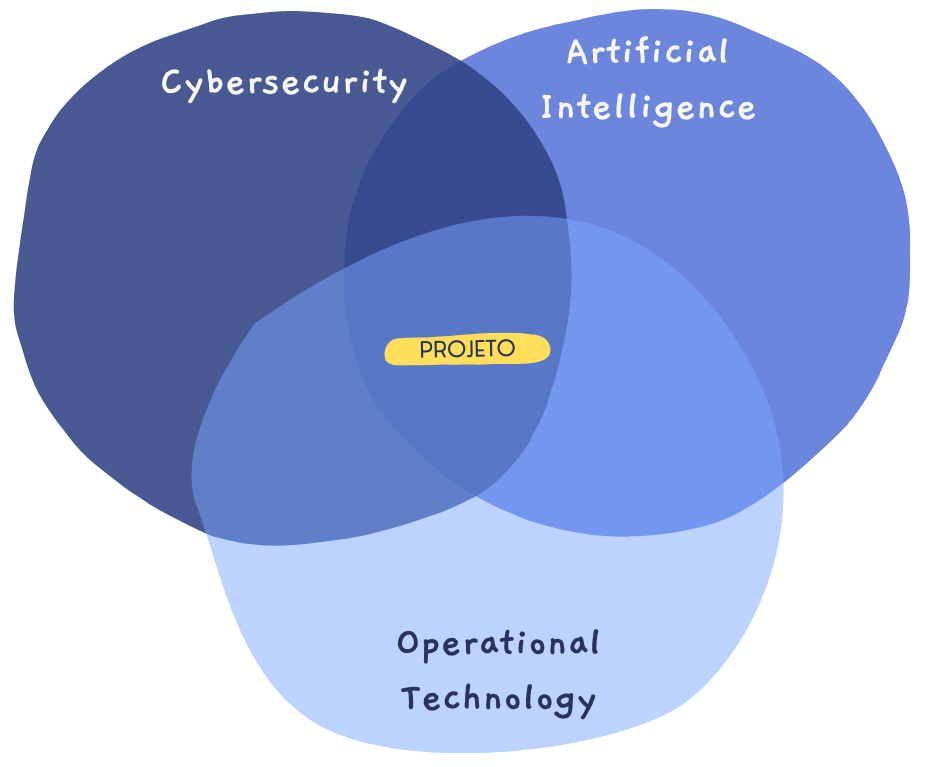
\includegraphics[scale=0.2]{triple.png}
                    \end{figure}
                }
            \end{column}
        \end{columns}
    \end{frame}

    \begin{frame}{Pesquisa bibliográfica}
        \begin{columns}
            \begin{column}{0.4\textwidth}
                \begin{wideitemize}
                    \item Bases de dados
                    \begin{wideitemize}
                        \item IEEEXplore
                        \item Scopus
                        \item Web Of Science
                    \end{wideitemize}
                    \item Termos de pesquisa
                    \begin{wideitemize}
                        \item \code{OPC UA}
                        \item \code{Intrusion Detection System}
                        \item \code{Machine Learning}
                        \item \code{Anomaly Detection}
                    \end{wideitemize}
                \end{wideitemize}
            \end{column}
            \begin{column}{0.6\textwidth}
                \begin{wideitemize}
                    \item Filtros de pesquisa
                    \begin{wideitemize}
                        \item \textbf{Idioma:} Inglês
                        \item \textbf{Data:} 2016 - 2023
                        \item \textbf{Busca:} Obrigatório o termo \code{OPC UA}
                    \end{wideitemize}
                    \item Principais referências
                    \begin{wideitemize}
                        \item Desenvolvimento de método para detecção de intrusão em redes PROFINET baseado em técnicas de Aprendizado de Máquina \cite{turcato2020}
                        \item Anomaly-based Intrusion Detection in Industrial Data with SVM and Random Forests \cite{anton2019}
                        \item Attack Detection in Cyber-Physical Production Systems using the Deterministic Dendritic Cell Algorithm \cite{pinto2020}
                    \end{wideitemize}
                \end{wideitemize}
            \end{column}
        \end{columns}
    \end{frame}

    \begin{frame}{Proposta}
        \begin{figure}
            \only<1>{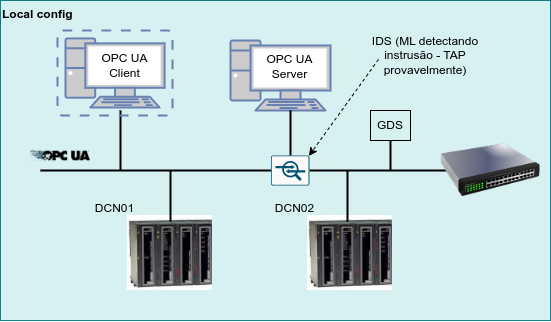
\includegraphics[scale=0.5]{local.png}}
            \only<2>{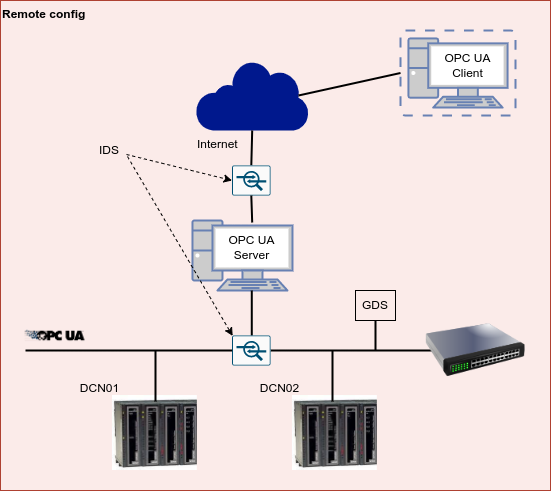
\includegraphics[scale=0.35]{remote.png}}
        \end{figure}
    \end{frame}

    \section{Metas estabelecidas}
    \begin{frame}
        \begin{table}[H]
            \caption{Metas estabelecidas para a pesquisa.}
            \label{tab:metas}
            \centering
            \begin{tabular}{
                |>{\centering\arraybackslash}m{0.075\textwidth}
                |>{\raggedright\arraybackslash}m{0.9\textwidth}
            |} \hline
                \thead{METAS} & \thead{DESCRIÇÃO} \\ \hline
                1 & Pesquisa bibliográfica \\ \hline
                2 & Projeto e implementação do ambiente de teste para coleta de dados \\ \hline
                3 & Implementar ataques no ambiente proposto \\ \hline
                4 & Coleta e tratamento dos dados (\textit{preprocessing}) \\ \hline
                5 & Apresentação para exame de qualificação \\ \hline
                6 & Análise das ferramentas de aprendizagem de máquinas \\ \hline
                7 & Desenvolvimento do método de detecção de intrusão\\ \hline
                8 & Verificação de desempenho e validação dos resultados \\ \hline
                9 & Escrita e submissão de artigo \\ \hline
                10 & Entrega final e defesa da dissertação \\
                \hline
            \end{tabular}
        \end{table}
    \end{frame}

    \subsection{Cronograma proposto}
    \begin{frame}
        \begin{table}[H]
            \centering
            \caption{Cronograma proposto para cumprimento das metas. }
            \label{tab:cronograma}
            \begin{tabular}{
                |>{\centering\arraybackslash}m{0.075\textwidth}
                |>{\centering\arraybackslash}m{0.045\textwidth}
                |>{\centering\arraybackslash}m{0.035\textwidth}
                |>{\centering\arraybackslash}m{0.035\textwidth}
                |>{\centering\arraybackslash}m{0.035\textwidth}
                |>{\centering\arraybackslash}m{0.035\textwidth}
                |>{\centering\arraybackslash}m{0.035\textwidth}
                |>{\centering\arraybackslash}m{0.035\textwidth}
                |>{\centering\arraybackslash}m{0.035\textwidth}
                |>{\centering\arraybackslash}m{0.035\textwidth}
                |>{\centering\arraybackslash}m{0.035\textwidth}
                |>{\centering\arraybackslash}m{0.035\textwidth}
                |>{\centering\arraybackslash}m{0.035\textwidth}
                |>{\centering\arraybackslash}m{0.035\textwidth}
                |>{\centering\arraybackslash}m{0.035\textwidth}
                |>{\centering\arraybackslash}m{0.035\textwidth}
                |>{\centering\arraybackslash}m{0.035\textwidth}
                |>{\centering\arraybackslash}m{0.035\textwidth}
                |>{\centering\arraybackslash}m{0.035\textwidth}
                |>{\centering\arraybackslash}m{0.035\textwidth}
            |} \hline
                \multicolumn{1}{|l|}{} & \textbf{2022} & \multicolumn{10}{c|}{\textbf{2023}} & \multicolumn{8}{c|}{\textbf{2024}} \\ \hline
                \textbf{METAS} & --              & 03 & 04 & 05 & 06 & 07 & 08 & 09 & 10 & 11 & 12 & 01 & 02 & 03 & 04 & 05 & 06 & 07 & 08 \\ \hline
                1    & \cellcolor{eescorange!30} & \y & \x & \x &    &    &    &    &    &    &    &    &    &    &    &    &    &    &    \\ \hhline{-~------------------}
                2    & \cellcolor{eescorange!30} &    & \x & \x & \x & \x & \x &    &    &    &    &    &    &    &    &    &    &    &    \\ \hhline{-~------------------}
                3    & \cellcolor{eescorange!30} &    &    &    & \x & \x & \x &    &    &    &    &    &    &    &    &    &    &    &    \\ \hhline{-~------------------}
                4    & \cellcolor{eescorange!30} &    &    & \x & \x & \x & \x & \x & \x &    &    &    &    &    &    &    &    &    &    \\ \hhline{-~------------------}
                5    & \cellcolor{eescorange!30} &    &    &    &    & \x & \x &    &    &    &    &    &    &    &    &    &    &    &    \\ \hhline{-~------------------}
                6    & \cellcolor{eescorange!30} &    &    &    & \x & \x & \x & \x & \x &    &    &    &    &    &    &    &    &    &    \\ \hhline{-~------------------}
                7    & \cellcolor{eescorange!30} &    &    &    &    &    &    & \x & \x & \x & \x & \x & \x & \x &    &    &    &    &    \\ \hhline{-~------------------}
                8    & \cellcolor{eescorange!30} &    &    &    &    &    &    &    &    &    &    &    & \x & \x & \x & \x &    &    &    \\ \hhline{-~------------------}
                9    & \cellcolor{eescorange!30} & \y & \y &    &    &    &    &    &    &    & \x & \x & \x & \x &    &    & \x & \x & \x \\ \hhline{-~------------------}
                10    & \cellcolor{eescorange!30}\multirow{-9}{*}{\rotatebox[origin=c]{90}{Disciplinas da pós-graduação}} &    &    &    &    &    &    &    &    &    &    &    &    &    &    &    &    & \x & \x \\ \hline
            \end{tabular}
            % \begin{flushleft}
            %     \includegraphics[scale=0.7]{Images/leg1.jpg}
            % \end{flushleft}
        \end{table}
    \end{frame}

	% \begin{frame}{Custom elements}
	% 	Normal text \alert{Alert Text}  \exemple{Example Text} \emph{Emphasis Text} \code{Code text}
	% 	\begin{columns}

	% 		\begin{column}{0.5\textwidth}

    %             \boxeesc{
	% 			\centering
	% 			A EESC box}

	% 			\begin{block}{Simple block}
	% 				\begin{itemize}
	% 					\item ...
	% 				\end{itemize}
	% 			\end{block}

	% 		\end{column}

	% 		\begin{column}{0.5\textwidth}
				
	% 			\begin{tcolorbox}[tableeesc, tabularx={X||Y|Y|Y}, boxrule=0.5pt, title=My price table, opacityback=0]
	% 				Color & Price 1  & Price 2  & Price 3 \\\hline\hline
	% 				Red   & 10.00   & 20.00   &  30.00 \\\hline
	% 				Green    & 20.00   & 30.00   &  40.00  \\\hline
	% 				Blue    & 30.00   & 40.00   &  50.00 \\\hline\hline
	% 				Orange  & 60.00   & 90.00   & 120.00 \\\hline
	% 			\end{tcolorbox}

	% 		\end{column}

	% 	\end{columns}
	% \end{frame}

    %________________________________________________________
    %-------------------- REFERENCES ------------------------

    \section*{References}
    \begin{frame}{Referências}
        \bibliographystyle{plain} % apalike
        \bibliography{references.bib}
    \end{frame}

    %________________________________________________________
    %-------------------- FINAL PAGE ------------------------

    {
        \usebackgroundtemplate{
\includegraphics[width=\paperwidth,height=\paperheight]{finalEESC.png}}
        \begin{frame}[plain]
        \end{frame}
    }
	% %________________________________________________________
	% %--------------------- OVERWIEW -------------------------

	% \section{Overview}
	% \begin{frame}{Overview}
	% 	Normal text \alert{Alert Text}  \exemple{Example Text} \emph{Emphasis Text}
	% 	\begin{columns}

	% 		\begin{column}{0.5\textwidth}

	% 			\begin{block}{Simple block}
	% 				\begin{itemize}
	% 					\item ...
	% 				\end{itemize}
	% 			\end{block}

	% 			\begin{exampleblock}{Example block}
	% 				\begin{itemize}
	% 					\item ...
	% 				\end{itemize}
	% 			\end{exampleblock}

	% 			\begin{alertblock}{Alert block}
	% 				\begin{itemize}
	% 					\item ...
	% 				\end{itemize}
	% 			\end{alertblock}
	% 		\end{column}

	% 		\begin{column}{0.5\textwidth}
	% 			\boxpurple{
	% 			\centering
	% 			A purple box}

	% 			\boxorange{
	% 			\centering
	% 			An orange box}

	% 			\boxgrey{
	% 			\centering
	% 			A gray box}

	% 			\begin{tcolorbox}[tablegreen,tabularx={X||Y|Y|Y|Y||Y}, boxrule=0.5pt, title=My price table]
	% 				Color & Price 1  & Price 2  & Price 3 \\\hline\hline
	% 				Red   & 10.00   & 20.00   &  30.00 \\\hline
	% 				Green    & 20.00   & 30.00   &  40.00  \\\hline
	% 				Blue    & 30.00   & 40.00   &  50.00 \\\hline\hline
	% 				Orange  & 60.00   & 90.00   & 120.00
	% 			\end{tcolorbox}
	% 		\end{column}

	% 	\end{columns}
	% \end{frame}

	% %________________________________________________________
	% %---------------------- BLOCKS --------------------------

	% \section{Blocks}
	% \begin{frame}{Blocks types}
	% 	\begin{block}{Simple block}
	% 		\begin{itemize}
	% 			\item First point
	% 			\item Second point
	% 			\item Third point
	% 		\end{itemize}
	% 	\end{block}

	% 	\begin{exampleblock}{}
	% 		Exemple block (without title)
	% 		\begin{itemize}
	% 			\item First point
	% 			\item Second point
	% 			\item Third point
	% 		\end{itemize}
	% 	\end{exampleblock}

	% 	\begin{alertblock}{\ }
	% 		Alert block (with a bar in title)
	% 		\begin{itemize}
	% 			\item First point
	% 			\item Second point
	% 			\item Third point
	% 		\end{itemize}
	% 	\end{alertblock}
	% \end{frame}

	% %________________________________________________________
	% %---------------------- BOXES ---------------------------

	% \section{Boxes}
	% \begin{frame}{Boxes}

	% 	\boxyellow{
	% 	\centering
	% 	...}

	% 	\boxorange{
	% 	\centering
	% 	...}

	% 	\boxbrown{
	% 	\centering
	% 	...}

	% 	\boxpurple{
	% 	\centering
	% 	...}

	% 	\boxblue{
	% 	\centering
	% 	...}

	% 	\boxgrey{
	% 	\centering
	% 	...}

	% 	\boxgreen{
	% 	\centering
	% 	...}

	% 	\boxblack{
	% 	\centering
	% 	...}

	% \end{frame}

	% %________________________________________________________
	% %---------------------- LISTS ---------------------------

	% \section{Lists}
	% 	\subsection{List items}
	% 	\begin{frame}{Items}

	% 		\begin{itemize}
	% 			\item ...
	% 			\item ...
	% 			\item ...
	% 		\end{itemize}
		
	% 	\end{frame} 

	% 	\subsection{Numbered list}
	% 	\begin{frame}{Numbered}

	% 		\begin{enumerate}
	% 			\item ...
	% 			\item ...
	% 			\item ...
	% 		\end{enumerate}
		
	% 	\end{frame} 

	% 	\subsection{Descriptive list} 
	% 	\begin{frame}{Descriptive} 

	% 		\begin{description}
	% 			\item [Theme 1:] ...
	% 			\item [Theme 2:] ...
	% 			\item [Theme 3:] ...
	% 		\end{description}

	% 	\end{frame}

	% %________________________________________________________
	% %---------------------- TABLES --------------------------

	% \section{Tables}
	% \begin{frame}{Tables 1}
	% 	\begin{columns}

	% 		\begin{column}{0.5\textwidth}  

	% 			\begin{tcolorbox}[tablered,tabularx={X||Y|Y}, boxrule=0.5pt, title=My price table]
	% 				Couleur & Prix 1  & Prix 2 \\\hline\hline
	% 				Rouge   & 10.00   & 20.00  \\\hline
	% 				Vert    & 20.00   & 30.00  \\\hline
	% 				Bleu    & 30.00   & 40.00  \\\hline\hline
	% 				Orange  & 60.00   & 90.00 
	% 			\end{tcolorbox}
				
	% 			\begin{tcolorbox}[tableorange,tabularx={X||Y|Y}, boxrule=0.5pt, title=My price table]
	% 				Couleur & Prix 1  & Prix 2 \\\hline\hline
	% 				Rouge   & 10.00   & 20.00  \\\hline
	% 				Vert    & 20.00   & 30.00  \\\hline
	% 				Bleu    & 30.00   & 40.00  \\\hline\hline
	% 				Orange  & 60.00   & 90.00 
	% 			\end{tcolorbox}
			
	% 		\end{column}

	% 		\begin{column}{0.5\textwidth}
		
	% 			\begin{tcolorbox}[tableblue,tabularx={X||Y|Y}, boxrule=0.5pt, title=My price table]
	% 				Couleur & Prix 1  & Prix 2 \\\hline\hline
	% 				Rouge   & 10.00   & 20.00  \\\hline
	% 				Vert    & 20.00   & 30.00  \\\hline
	% 				Bleu    & 30.00   & 40.00  \\\hline\hline
	% 				Orange  & 60.00   & 90.00 
	% 			\end{tcolorbox}
				
	% 			\begin{tcolorbox}[tableyellow,tabularx={X||Y|Y}, boxrule=0.5pt, title=My price table]
	% 				Couleur & Prix 1  & Prix 2 \\\hline\hline
	% 				Rouge   & 10.00   & 20.00  \\\hline
	% 				Vert    & 20.00   & 30.00  \\\hline
	% 				Bleu    & 30.00   & 40.00  \\\hline\hline
	% 				Orange  & 60.00   & 90.00 
	% 			\end{tcolorbox}
				
	% 		\end{column}

	% 	\end{columns}
	% \end{frame}
	
	% \begin{frame}{Tables 2}
	% 	\begin{columns}

	% 		\begin{column}{0.5\textwidth} 
			
	% 			\begin{tcolorbox}[tablegrey,tabularx={X||Y|Y}, boxrule=0.5pt, title=My price table]
	% 				Couleur & Prix 1  & Prix 2 \\\hline\hline
	% 				Rouge   & 10.00   & 20.00  \\\hline
	% 				Vert    & 20.00   & 30.00  \\\hline
	% 				Bleu    & 30.00   & 40.00  \\\hline\hline
	% 				Orange  & 60.00   & 90.00 
	% 			\end{tcolorbox}
				
	% 			\begin{tcolorbox}[tablebrown,tabularx={X||Y|Y}, boxrule=0.5pt, title=My price table]
	% 				Couleur & Prix 1  & Prix 2 \\\hline\hline
	% 				Rouge   & 10.00   & 20.00  \\\hline
	% 				Vert    & 20.00   & 30.00  \\\hline
	% 				Bleu    & 30.00   & 40.00  \\\hline\hline
	% 				Orange  & 60.00   & 90.00 
	% 			\end{tcolorbox}

	% 		\end{column}

	% 		\begin{column}{0.5\textwidth}  

	% 			\begin{tcolorbox}[tablepurple,tabularx={X||Y|Y}, boxrule=0.5pt, title=My price table]
	% 				Couleur & Prix 1  & Prix 2 \\\hline\hline
	% 				Rouge   & 10.00   & 20.00  \\\hline
	% 				Vert    & 20.00   & 30.00  \\\hline
	% 				Bleu    & 30.00   & 40.00  \\\hline\hline
	% 				Orange  & 60.00   & 90.00 
	% 			\end{tcolorbox}
				
	% 			\begin{tcolorbox}[tableblack,tabularx={X||Y|Y}, boxrule=0.5pt, title=My price table]
	% 				Couleur & Prix 1  & Prix 2 \\\hline\hline
	% 				Rouge   & 10.00   & 20.00  \\\hline
	% 				Vert    & 20.00   & 30.00  \\\hline
	% 				Bleu    & 30.00   & 40.00  \\\hline\hline
	% 				Orange  & 60.00   & 90.00 
	% 			\end{tcolorbox}

	% 		\end{column}

	% 	\end{columns}
	% \end{frame}
	
	% \begin{frame}{Tables 3}
	% 	\centering
	% 	\begin{tcolorbox}[tableeesc, tabularx={XXYYYYZZ}, boxrule=0.5pt, title=USP custom table, opacityback=0]
	% 		\hline
	% 		{$m$} & {$\Re\{\underline{\mathfrak{X}}(m)\}$} & {$-\Im\{\underline{\mathfrak{X}}(m)\}$} & {$\mathfrak{X}(m)$} & {$\frac{\mathfrak{X}(m)}{23}$} & {$A_m$} & {$\varphi(m)\ /\ ^{\circ}$} & {$\varphi_m\ /\ ^{\circ}$} \\ \hline
	% 		1  & 16.128 & +8.872 & 16.128 & 1.402 & 1.373 & -146.6 & -137.6 \\
	% 		2  & 3.442  & -2.509 & 3.442  & 0.299 & 0.343 & 133.2  & 152.4  \\
	% 		3  & 1.826  & -0.363 & 1.826  & 0.159 & 0.119 & 168.5  & -161.1 \\
	% 		4  & 0.993  & -0.429 & 0.993  & 0.086 & 0.08  & 25.6   & 90     \\ \hline
	% 		5  & 1.29   & +0.099 & 1.29   & 0.112 & 0.097 & -175.6 & -114.7 \\
	% 		6  & 0.483  & -0.183 & 0.483  & 0.042 & 0.063 & 22.3   & 122.5  \\
	% 		7  & 0.766  & -0.475 & 0.766  & 0.067 & 0.039 & 141.6  & -122   \\
	% 		8  & 0.624  & +0.365 & 0.624  & 0.054 & 0.04  & -35.7  & 90     \\ \hline
	% 		9  & 0.641  & -0.466 & 0.641  & 0.056 & 0.045 & 133.3  & -106.3 \\
	% 		10 & 0.45   & +0.421 & 0.45   & 0.039 & 0.034 & -69.4  & 110.9  \\
	% 		11 & 0.598  & -0.597 & 0.598  & 0.052 & 0.025 & 92.3   & -109.3 \\ \hline
	% 	\end{tcolorbox}
	% \end{frame}

	% %________________________________________________________
	% %--------------------- FIGURES --------------------------

	% \section{Figures}
	% \begin{frame}{Figure Example} 
	% 	\begin{figure}
	% 		\centering
	% 		
\includegraphics[scale=0.1]{titleEESC.png}
	% 		\caption{System302 é o sistema da \cref{https://www.smar.com/pt}{SMAR}.}
	% 	\end{figure}
	% \end{frame}

	% %________________________________________________________
	% %----------------- EQUATIONS & CODES --------------------
	
	% \section{Equations and Codes}
	% 	\subsection{Equations}

	% 	\begin{frame}
	% 	\frametitle{Equation Example}

	% 		\begin{block}{Some random equation:}
	% 			\begin{align*}
	% 				\frac{\partial}{\partial \theta_k}J(\theta) 
	% 					&= \frac{\partial}{\partial \theta_k}\Bigg[\frac{1}{m}\sum_{k=1}^m log(1+e^{-y^{(i)}\theta^Tx^{(i)}})\Bigg] \\
	% 					&= \frac{1}{m}\sum_{k=1}^m \frac{1}{1+e^{-y^{(i)}\theta^Tx^{(i)}}}y^{(i)}x_k^{(i)} \\
	% 					&= -\frac{1}{m}\sum_{k=1}^m h_\theta(-y^{(i)}x^{(i)})y^{(i)}x_k^{(i)}        
	% 			\end{align*}
	% 		\end{block}

	% 	\end{frame}

	% 	\subsection{Programming}
	% 	\begin{frame}[fragile]
	% 	\frametitle{Code Example \#1}

	% 		\begin{figure}
	% 			\centering
	% 			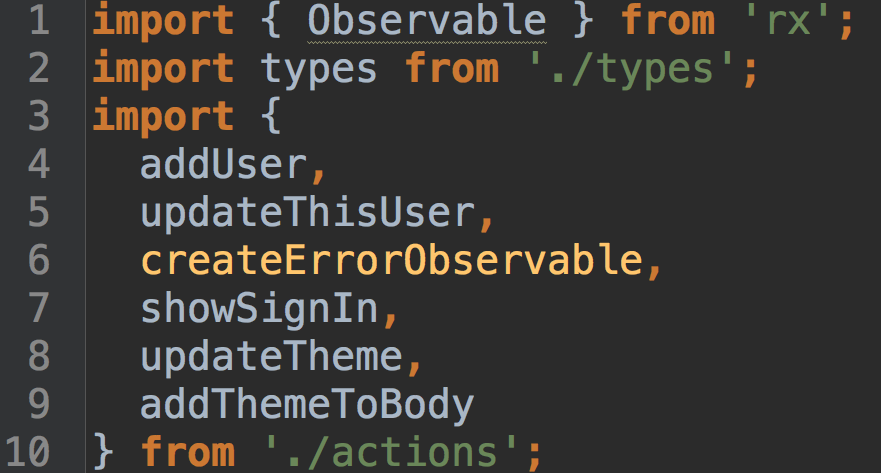
\includegraphics[width=0.8\linewidth]{code.png}
	% 		\end{figure}
	% 		\blfootnote{\href{https://miro.medium.com/max/881/1*SKIAmwDYVnrMvFOopOCwPQ.png}{Code}}

	% 	\end{frame}

	% 	\begin{frame}[fragile]
	% 	\frametitle{Code Example \#2}
		
	% 		\codebox{\textbf{import} numpy \textbf{as} np}

	% 		\begin{lstlisting}[language=Python]
	% 			def code():
	% 			# test comments #1    
	% 			if True:
	% 				for _ in range(5):
	% 				print("Hello World 5 times")
	% 			return None     
	% 		\end{lstlisting}

	% 	\end{frame}

	% %________________________________________________________
	% %--------------------- ANIMATIONS -----------------------
	
	% % \begin{frame}{Schedule}
	% % 	\tableofcontents[part=2]
	% % \end{frame}

	% \section{Animations}

	% 	\begin{frame}
	% 	\frametitle{Pause}
	% 		\begin{itemize}
	% 			\item I'm going to put here some elements with purpose to show the presentation pause effect. \pause
	% 			\item The next item only display... \pause
	% 			\item If you interact with it.
	% 		\end{itemize} \pause

	% 		\begin{block}{Some random equation:}
	% 			\begin{align*}
	% 				\frac{\partial}{\partial \theta_k}J(\theta)
	% 					&= \frac{\partial}{\partial \theta_k}\Bigg[\frac{1}{m}\sum_{k=1}^m log(1+e^{-y^{(i)}\theta^Tx^{(i)}})\Bigg] \\ \pause
	% 					&= \frac{1}{m}\sum_{k=1}^m \frac{1}{1+e^{-y^{(i)}\theta^Tx^{(i)}}}y^{(i)}x_k^{(i)} \\ \pause
	% 					&= -\frac{1}{m}\sum_{k=1}^m h_\theta(-y^{(i)}x^{(i)})y^{(i)}x_k^{(i)}   
	% 			\end{align*}
	% 		\end{block}
	% 	\end{frame}

	% 	\subsection{Contents overlay}
	% 	\begin{frame}
	% 		\frametitle{Uncover}
	% 		\uncover<-3,5>{Let's solve a quadratic equation: $$ax^2 + bx + c = 0$$}
	% 		\uncover<2-4>{First you need to identify the coefficients $a$, $b$ and $c$.}
	% 		\uncover<3->{Then calculate the value of: $$\Delta = b^2 - 4ac$$}
	% 		\uncover<4>{Calculate the first root: $$x_1 = \frac{-b + \sqrt{\Delta}}{2a}$$}
	% 		\uncover<5>{Calculate the second root: $$x_1 = \frac{-b - \sqrt{\Delta}}{2a}$$}
	% 	\end{frame}

	% 	\begin{frame}
	% 		\frametitle{Visible}
	% 		\visible<1>{Let's solve a quadratic equation: $$ax^2 + bx + c = 0$$}
	% 		\visible<2>{First you need to identify the coefficients $a$, $b$ and $c$.}
	% 		\visible<3>{Then calculate the value of: $$\Delta = b^2 - 4ac$$}
	% 		\visible<4>{Calculate the first root: $$x_1 = \frac{-b + \sqrt{\Delta}}{2a}$$}
	% 		\visible<5>{Calculate the second root: $$x_1 = \frac{-b - \sqrt{\Delta}}{2a}$$}
	% 	\end{frame}

	% 	\begin{frame}
	% 		\frametitle{Only}
	% 		\only<1>{Let's solve a quadratic equation: $$ax^2 + bx + c = 0$$}
	% 		\only<2>{First you need to identify the coefficients $a$, $b$ and $c$.}
	% 		\only<3>{Then calculate the value of: $$\Delta = b^2 - 4ac$$}
	% 		\only<4>{Calculate the first root: $$x_1 = \frac{-b + \sqrt{\Delta}}{2a}$$}
	% 		\only<5>{Calculate the second root: $$x_1 = \frac{-b - \sqrt{\Delta}}{2a}$$}
	% 	\end{frame}

	% 	\subsection{Environments actions}
	% 	\begin{frame}
	% 		\frametitle{Alert}
	% 		\begin{itemize}
	% 			\item<1- | alert@1> Let's solve a quadratic equation: $$ax^2 + bx + c = 0$$
	% 			\item<2- | alert@2> First you need to identify the coefficients $a$, $b$ and $c$.
	% 			\item<3- | alert@3> Then calculate the value of: $$\Delta = b^2 - 4ac$$
	% 			\item<4- | alert@4> Calculate the first root: $$x_1 = \frac{-b + \sqrt{\Delta}}{2a}$$
	% 			\item<5- | alert@5> Calculate the second root: $$x_1 = \frac{-b - \sqrt{\Delta}}{2a}$$
	% 		\end{itemize}
	% 	\end{frame}

	% 	\begin{frame}
	% 		\frametitle{Alert - optimized}
	% 		\begin{itemize}[<+- | alert@+>] % uncover, visible and only
	% 			\item Let's solve a quadratic equation: $$ax^2 + bx + c = 0$$
	% 			\item First you need to identify the coefficients $a$, $b$ and $c$.
	% 			\item Then calculate the value of: $$\Delta = b^2 - 4ac$$
	% 			\item Calculate the first root: $$x_1 = \frac{-b + \sqrt{\Delta}}{2a}$$
	% 			\item Calculate the second root: $$x_1 = \frac{-b - \sqrt{\Delta}}{2a}$$
	% 		\end{itemize}
	% 	\end{frame}

	% 	%________________________________________________________
	% 	%--------------------- NAVIGATION -----------------------

	% 	\section{Navigation}
	% 	\subsection{Links and Buttons}

	% 	\begin{frame}
	% 		\frametitle{Navigation frame 1}

	% 		\hyperlink{fra:navSlide2}{\beamerbutton{Slide 2 (Frame 3)}}
	% 		\hyperlink{fra:navSlide3}{\beamergotobutton{Slide 3 (Frame 2)}}
	% 		\hyperlink{fra:navSlide2}{\beamerskipbutton{Slide 2 (Frame 3)}}
	% 		\hyperlink{fra:navSlide3}{\beamerreturnbutton{Slide 3 (Frame 2)}}

	% 		\hyperlinkslidenext{\beamergotobutton{Next Slide}}
	% 		\hyperlinkslideprev{\beamergotobutton{Previous Slide}}
			
	% 		\hyperlinkpartstart{\beamerbutton{Start of part}}
	% 		\hyperlinkpartend{\beamerbutton{End of part}}
	% 		\hyperlinksectionstart{\beamerbutton{Start of section}}
	% 		\hyperlinksectionend{\beamerbutton{End of section}}
	% 		\hyperlinkframestart{\beamerbutton{Start of frame}}
	% 		\hyperlinkframeend{\beamerbutton{End of frame}} % Também há para subseção, capítulo...

	% 		\hyperlinkframestartnext{\beamerskipbutton{Start of the next frame}}
	% 		\hyperlinkframeendprev{\beamerskipbutton{End of the next frame}} % Também tem o apêndice

	% 		\hyperlinkpresentationstart{\beamerreturnbutton{Start of presentation}} \hyperlinkpresentationend{\beamerskipbutton{End of presentation}} % Também tem o document
	% 	\end{frame}

	% 	\begin{frame}
	% 		\frametitle{Navigation frame 2}

	% 		\begin{itemize}
	% 			\item<1-> Slide 1
	% 			\item<2-> Slide 2
	% 			\item<3-> Slide 3
	% 			\item<4-> Slide 4
	% 		\end{itemize}
	% 		\hypertarget<3>{fra:navSlide3}{}
	% 		\hyperlink{fra:navFrame3<4>}{Slide 4 (Frame 3)}
	% 	\end{frame}

	% 	\begin{frame}<1-2>[label=fra:navFrame3]
	% 		\frametitle{Navigation frame 3}
	% 		\begin{itemize}
	% 			\item<1-> Slide 1
	% 			\item<2-> Slide 2
	% 			\item<3-> Slide 3
	% 			\item<4-> Slide 4
	% 		\end{itemize}
	% 		\hypertarget<2>{fra:navSlide2}{}
	% 	\end{frame}

	% 	\begin{frame}
	% 		\frametitle{Navigation frame 4}
	% 		\begin{itemize}
	% 			\item<1-> Slide 1
	% 			\item<2-> Slide 2
	% 			\item<3-> Slide 3
	% 			\item<4-> Slide 4
	% 		\end{itemize}
	% 	\end{frame}

	% 	\againframe<3->{fra:navFrame3}
	% 	\subsection{Zoom}
	% 	\begin{frame}<1>[label=fra:zooms]{Zoom Example}
	% 		\hypersetup{linkbordercolor=yellow}
	% 		\framezoom<1><2>[border=2](4.6cm, 0.6cm)(4.6cm, 2.2cm)
	% 		\framezoom<1><3>[border=2](5.0cm, 3cm)(3.9cm, 1cm)
	% 		\begin{figure}
	% 			\centering
	% 			
\includegraphics[scale=0.1]{titleEESC.png}
	% 			\caption{System302 é o sistema da \cref{https://www.smar.com/pt}{SMAR}.}
	% 		\end{figure}
	% 	\end{frame}

	% 	\subsection{Multimedia}

	% 	\begin{frame}{Video}
	% 		\centering
	% 		\movie[width=160px, 
	% 			height=90px,
	% 			%externalviewer,
	% 			%loop,
	% 			showcontrols,
	% 			poster
	% 		]{Watch}{Public/Videos/videoDemo.mp4} % Add option "" to watch in a external viewer
	% 		%\movie[width=160px, height=90px]{\includegraphics[]{}}{Public/Videos/videoDemo.mp4}
	% 	\end{frame}

	% 	\begin{frame}{Sound}
	% 		\sound[%inlinesound, % Arquivo vai ser copiado dentro do próprio PDF, sem precisar de arquivo externo
	% 			%loop,
	% 			%mixsound=true,
	% 		]{Listen}{Public/Sounds/soundDemo.mp3}
	% 	\end{frame}

	% 	\newcount\countName
	% 	\newdimen\dimName

	% 	\begin{frame}{Transiction}
	% 		\animate<1->
	% 		\animatevalue<1-4>{\countName}{0}{100}
	% 		\animatevalue<1-4>{\dimName}{0cm}{8cm}

	% 		\textcolor{red!\the\countName!black}{Aqui vem um texto.}

	% 		{\hspace{\dimName} Aqui vem outro texto}

	% 		\begin{itemize}
	% 			\item<1-> Slide 1
	% 			\item<2-> Slide 2
	% 			\item<3-> Slide 3
	% 			\item<4-> Slide 4
	% 		\end{itemize}
	% 	\end{frame}

	% 	\begin{frame}[fragile]{Transition}
	% 		\transdissolve[duration=2]<2>
	% 		\transblindshorizontal<3>
	% 		\transboxin<4>
	% 		\transglitter[duration=2, direction=180]<5>
	% 		\begin{itemize}
	% 			\item<1-> Slide 1 citation \cite{gratzer2007more}
	% 			\item<2-> Slide 2 citation \cite{kottwitz2021latex}
	% 			\item<3-> Slide 3 citation \cite{mittelbach2004latex}
	% 			\item<4-> Slide 4 citation \cite{martin2009clean}
	% 			\item<5-> A few more transitions: 
				
	% 			\verb=\transblindsvertical<4>, \transboxout<6>, \transsplitverticalin, \transsplitverticalout=
	% 			\verb=\transsplithorizontalin, \transsplithorizontalout, \transwipe=
	% 		\end{itemize}
	% 	\end{frame}

	% 	\begin{frame}[fragile=singleslide]{Citation}
		
	% 		A few more options for the \verb=\cite= command in \textbf{NATBIB} are available:

	% 		\begin{table}
	% 			\centering
	% 			\begin{tabular}{l l}
	% 				\hline
	% 				Command & Output \\
	% 				\hline
	% 				\verb=\citet{key}= & Jones et al. (1990) \\
	% 				\verb=\citealt{key}= & Jones et al.'s 1990 \\
	% 				\verb=\citet*{key}= & Jones, Baker, and Smith (1990) \\
	% 				\verb=\citep{key}= & (Jones et al. 1990) \\
	% 				\verb=\citep*{key}= & (Jones, Baker, and Smith 1990) \\
	% 				\verb=\citep[p.~99]{key}= & (Jones et al., 1990, p. 99) \\
	% 				\verb=\citep[e.g.][]{key}= & (e.g. Jones et al., 1990) \\
	% 				\verb=\citep[e.g.][p.~99]{key}= & (e.g. Jones et al., 1990, p. 99) \\
	% 				\verb=\citeauthor{key}= & Jones et al. \\
	% 				\verb=\citeauthor*{key}= & Jones, Baker, and Smith \\
	% 				\verb=\citeyear{key}= & 1990 \\
	% 				\verb=\citeapos{key}*= & Jones et al.'s (1990) \\
	% 				\hline
	% 			\end{tabular}
	% 		\end{table}
	% 	\end{frame}

\end{document}